\begin{landscape}
\section{Appendix}
\subsection{Speech Recognition Results} \label{sec:appendix}

Table \ref{tab:en-short} shows a task-breakdown of short-form English speech recognition results for LibriSpeech Test Clean \citep{panayotov15_librispeech}, LibriSpeech Test Other, GigaSpeech \citep{chen21_gigaspeech}, VoxPopuli \citep{wang21_voxpopuli}, SwitchBoard \citep{godfrey92_switchboard}, CallHome, CHiME-4 \citep{chime4_17}, SPGISpeech \citep{oneill21_spgispeech}, TED-LIUM \citep{Hernandez_2018Tedlium} and Earnings-22 \citep{delrio22_earnings22}. % For GigaSpeech and SPGISpeech, we use a random subset of 2k datapoints to enable evaluating the Realtime APIs.

\begin{table}[h]
\centering
\caption{English Short-Form WER (\%) results. We report scores for LibriSpeech Test Clean (LS-C), LibriSpeech Test Other (LS-O), GigaSpeech (GS), VoxPopuli (VP), SwitchBoard (SB), CallHome (CH), CHiME-4 (C-4), SPGISPeech (SPGI), TED-LIUM (TED) and Earnings-22 (E22).}
\label{tab:en-short}
\small
\begin{tabular}{lcccccccccccc}
\toprule
\textbf{Model} & \textbf{Delay (ms)} & \textbf{LS-C} & \textbf{LS-O} & \textbf{GS} & \textbf{VP} & \textbf{SB} & \textbf{CH} & \textbf{C-4} & \textbf{SPGI} & \textbf{TED} & \textbf{E22} & \textbf{AVG} \\
\midrule

\multicolumn{13}{l}{\textit{Offline}} \\
\cmidrule(lr){1-13}
Whisper & — & 1.84 & 3.66 & 11.60 & 9.58 & 13.14 & 14.58 & 10.88 & 3.15 & 3.83 & 11.63 & 8.39 \\
Voxtral Mini Transcribe V2 & — & 1.60 & 3.24 & 10.39 & 6.81 & 11.54 & 12.74 & 10.42 & 1.74 & 3.50 & 10.67 & 7.27 \\

\addlinespace[0.6em]
\multicolumn{13}{l}{\textit{Realtime API}} \\
\cmidrule(lr){1-13}
GPT-4o mini Transcribe & — & 1.94 & 4.48 & 10.67 & 6.79 & 11.15 & 15.54 & 11.08 & 2.87 & 4.07 & 10.69 & 7.93 \\
Scribe v2 Realtime & — & 1.75 & 4.01 & 10.29 & 6.01 & 11.54 & 11.87 & 11.59 & 2.04 & 2.63 & 11.52 & 7.33 \\

\addlinespace[0.6em]
\multicolumn{13}{l}{\textit{Realtime Open-Source}} \\
\cmidrule(lr){1-13}
DSM 1B En-Fr & 500 & 3.64 & 11.44 & 12.09 & 11.51 & 12.46 & 16.62 & 28.84 & 4.63 & 4.58 & 16.76 & 12.26 \\
DSM 2.6B En & 2500 & 1.71 & 4.46 & 10.39 & 6.51 & 12.53 & 12.02 & 16.75 & 1.95 & 3.08 & 11.72 & 8.11 \\
\addlinespace
\multirow[t]{2}{*}{Nemotron Streaming} & 560 & 2.42 & 5.12 & 11.87 & 7.09 & 13.82 & 17.30 & 18.64 & 2.64 & 4.50 & 12.48 & 9.59 \\
 & 1120 & 2.38 & 4.94 & 11.84 & 7.02 & 13.35 & 17.74 & 17.37 & 2.62 & 4.50 & 12.33 & 9.41 \\
\addlinespace
\multirow[t]{4}{*}{Voxtral Realtime} & 240 & 2.49 & 7.15 & 12.10 & 10.52 & 13.26 & 14.66 & 18.07 & 3.31 & 4.53 & 13.39 & 9.95 \\
 & 480 & 2.08 & 5.54 & 11.05 & 7.87 & 11.90 & 13.59 & 15.00 & 1.96 & 3.96 & 11.71 & 8.47 \\
 & 960 & 1.96 & 4.59 & 10.51 & 7.23 & 11.44 & 13.34 & 13.17 & 2.36 & 3.55 & 11.24 & 7.94 \\
 & 2400 & 1.82 & 4.03 & 10.60 & 7.06 & 11.55 & 13.44 & 12.18 & 2.11 & 3.57 & 10.80 & 7.72 \\
\bottomrule
\end{tabular}
\end{table}



For English long-form, we report Meanwhile \citep{radford2023whisper} and the long-form version of TED-LIUM. We also take the one-hour long earnings calls from Earnings-21 \citep{delrio21_earnings21} and Earnings-22 \citep{delrio22_earnings22}, and segment them into shorter, 10 minute variants.

\begin{table}[h]
\centering
\caption{English Long-Form WER (\%) results. We report scores for Meanwhile (MW), Earnings-21 (E21), Earnings-22 (E22), and TED-LIUM (TED).}
\label{tab:en-long}
\small
\begin{tabular}{lcccccc}
\toprule
\textbf{Model} & \textbf{Delay (ms)} & \textbf{MW} & \textbf{E21} & \textbf{E22} & \textbf{TED} & \textbf{AVG} \\
\midrule

\multicolumn{7}{l}{\textit{Offline}} \\
\cmidrule(lr){1-7}
Whisper & — & 5.80 & 9.88 & 13.07 & 3.11 & 7.97 \\
Voxtral Mini Transcribe V2 & — & 4.08 & 9.81 & 11.69 & 2.86 & 7.11 \\

\addlinespace[0.6em]
\multicolumn{7}{l}{\textit{Realtime API}} \\
\cmidrule(lr){1-7}
GPT-4o mini Transcribe & — & 5.21 & 9.92 & 12.58 & 4.17 & 7.97 \\
Scribe v2 Realtime & — & 3.62 & 10.72 & 13.22 & 2.18 & 7.43 \\

\addlinespace[0.6em]
\multicolumn{7}{l}{\textit{Realtime Open-Source}} \\
\cmidrule(lr){1-7}
DSM 1B En-Fr & 500 & 7.36 & 14.58 & 21.43 & 11.92 & 13.83 \\
DSM 2.6B En & 2500 & 5.29 & 10.52 & 12.18 & 2.89 & 7.72 \\
\addlinespace
\multirow[t]{2}{*}{Nemotron Streaming} & 560 & 8.25 & 20.92 & 23.53 & 4.46 & 14.29 \\
 & 1120 & 7.43 & 18.75 & 21.65 & 4.25 & 13.02 \\
\addlinespace
\multirow[t]{4}{*}{Voxtral Realtime} & 240 & 5.76 & 12.56 & 14.84 & 4.00 & 9.29 \\
 & 480 & 5.05 & 10.46 & 12.46 & 2.94 & 7.73 \\
 & 960 & 4.14 & 9.86 & 11.63 & 2.86 & 7.13 \\
 & 2400 & 4.03 & 9.52 & 11.31 & 2.86 & 6.93 \\
\bottomrule
\end{tabular}
\end{table}


Tables \ref{tab:fleurs} and \ref{tab:mcv} show the per-language breakdown of error-rate scores for the FLEURS and Mozilla Common Voice benchmarks respectively.

\begin{table}[h]
\centering
\caption{FLEURS error-rate results by language. We report scores for Arabic (ar), German (de), English (en), Spanish (es), French (fr), Hindi (hi), Italian (it), Japanese (ja), Korean (ko), Dutch (nl), Portuguese (pt), Russian (ru), and Chinese (zh). For Chinese and Japanese we report character error-rate (CER). For all other languages, we report WER.}
\label{tab:fleurs}
\small
\begin{tabular}{lccccccccccccccc}
\toprule
\textbf{Model} & \textbf{Delay (ms)} & \textbf{ar} & \textbf{de} & \textbf{en} & \textbf{es} & \textbf{fr} & \textbf{hi} & \textbf{it} & \textbf{ja} & \textbf{ko} & \textbf{nl} & \textbf{pt} & \textbf{ru} & \textbf{zh} & \textbf{AVG} \\
\midrule

\multicolumn{16}{l}{\textit{Offline}} \\
\cmidrule(lr){1-16}
Whisper & — & 15.44 & 5.46 & 4.00 & 2.81 & 5.55 & 28.87 & 2.71 & 4.97 & 14.30 & 5.87 & 3.90 & 5.13 & 7.94 & 8.23 \\
Voxtral Mini Transcribe V2 & — & 13.54 & 3.54 & 3.32 & 2.63 & 4.32 & 10.33 & 2.17 & 4.14 & 12.29 & 4.78 & 3.56 & 4.75 & 7.30 & 5.90 \\

\addlinespace[0.6em]
\multicolumn{16}{l}{\textit{Realtime API}} \\
\cmidrule(lr){1-16}
GPT-4o mini Transcribe & — & 13.99 & 4.07 & 3.65 & 3.41 & 5.84 & 8.39 & 2.82 & 9.89 & 19.46 & 6.00 & 5.04 & 5.30 & 15.43 & 7.95 \\
Scribe v2 Realtime & — & 19.53 & 4.31 & 3.54 & 3.23 & 5.12 & 12.62 & 2.33 & 10.92 & 11.90 & 6.72 & 3.75 & 7.68 & 16.82 & 8.34 \\

\addlinespace[0.6em]
\multicolumn{16}{l}{\textit{Realtime Open-Source}} \\
\cmidrule(lr){1-16}
DSM 1B En-Fr & 500 & — & — & 9.56 & — & 16.31 & — & — & — & — & — & — & — & — & — \\
DSM 2.6B En & 2500 & — & — & 6.11 & — & — & — & — & — & — & — & — & — & — & — \\
\addlinespace
\multirow[t]{2}{*}{Nemotron Streaming} & 560 & — & — & 6.11 & — & — & — & — & — & — & — & — & — & — & — \\
 & 1120 & — & — & 5.72 & — & — & — & — & — & — & — & — & — & — & — \\
\addlinespace
\multirow[t]{4}{*}{Voxtral Realtime} & 240 & 23.95 & 8.15 & 5.91 & 4.59 & 8.00 & 14.26 & 4.41 & 15.17 & 17.56 & 9.23 & 7.51 & 7.87 & 13.84 & 10.80 \\
 & 480 & 22.53 & 6.19 & 4.90 & 3.31 & 6.42 & 12.88 & 3.27 & 9.59 & 15.74 & 7.07 & 5.03 & 6.02 & 10.45 & 8.72 \\
 & 960 & 20.32 & 4.87 & 4.34 & 2.98 & 5.68 & 11.82 & 2.46 & 6.80 & 14.90 & 6.76 & 4.57 & 5.56 & 8.99 & 7.70 \\
 & 2400 & 14.71 & 4.15 & 4.05 & 2.71 & 5.23 & 10.73 & 2.37 & 5.50 & 14.30 & 5.91 & 3.93 & 5.41 & 8.48 & 6.73 \\
\bottomrule
\end{tabular}
\end{table}


\begin{table}[h]
\centering
\caption{Mozilla Common Voice error-rate results by language. For Chinese and Japanese we report CER. For all other languages, we report WER. For fairness, we omit Arabic from the macro-average in Tables~\ref{tab:results} and~\ref{tab:left-padding}, since all models score in excess of 45\%.}
\label{tab:mcv}
\small
\begin{tabular}{lccccccccccccccc}
\toprule
\textbf{Model} & \textbf{Delay (ms)} & \textbf{ar} & \textbf{de} & \textbf{en} & \textbf{es} & \textbf{fr} & \textbf{hi} & \textbf{it} & \textbf{ja} & \textbf{ko} & \textbf{nl} & \textbf{pt} & \textbf{ru} & \textbf{zh} & \textbf{AVG} \\
\midrule

\multicolumn{16}{l}{\textit{Offline}} \\
\cmidrule(lr){1-16}
Whisper & — & 50.58 & 6.25 & 22.91 & 5.66 & 11.33 & 46.75 & 6.81 & 15.80 & 20.86 & 5.83 & 7.17 & 6.76 & 14.88 & 14.25 \\
Voxtral Mini Transcribe V2 & — & 46.06 & 4.35 & 8.61 & 3.93 & 7.21 & 10.26 & 4.15 & 12.87 & 20.29 & 4.38 & 6.58 & 5.18 & 9.04 & 8.07 \\

\addlinespace[0.6em]
\multicolumn{16}{l}{\textit{Realtime API}} \\
\cmidrule(lr){1-16}
GPT-4o mini Transcribe & — & 51.06 & 6.05 & 10.89 & 5.54 & 9.77 & 23.90 & 5.75 & 18.53 & 32.90 & 7.89 & 9.70 & 8.49 & 14.81 & 12.85 \\
Scribe v2 Realtime & — & 60.60 & 16.60 & 19.43 & 15.93 & 15.74 & 35.78 & 14.04 & 24.70 & 26.98 & 9.06 & 19.77 & 13.16 & 38.97 & 20.85 \\

\addlinespace[0.6em]
\multicolumn{16}{l}{\textit{Realtime Open-Source}} \\
\cmidrule(lr){1-16}
DSM 1B En-Fr & 500 & — & — & 34.93 & — & 24.29 & — & — & — & — & — & — & — & — & — \\
DSM 2.6B En & 2500 & — & — & 18.27 & — & — & — & — & — & — & — & — & — & — & — \\
\addlinespace
\multirow[t]{2}{*}{Nemotron Streaming} & 560 & — & — & 12.33 & — & — & — & — & — & — & — & — & — & — & — \\
 & 1120 & — & — & 11.92 & — & — & — & — & — & — & — & — & — & — & — \\
\addlinespace
\multirow[t]{4}{*}{Voxtral Realtime} & 240 & 55.10 & 11.13 & 19.63 & 9.05 & 14.51 & 20.05 & 10.62 & 27.25 & 33.47 & 11.86 & 15.27 & 13.90 & 43.93 & 19.22 \\
 & 480 & 48.64 & 8.70 & 15.18 & 6.05 & 11.51 & 17.22 & 7.80 & 20.87 & 31.37 & 8.97 & 11.25 & 11.03 & 32.92 & 15.24 \\
 & 960 & 48.68 & 6.85 & 12.49 & 5.12 & 9.80 & 15.04 & 6.05 & 16.77 & 27.24 & 6.36 & 8.00 & 8.65 & 21.51 & 11.99 \\
 & 2400 & 50.35 & 5.66 & 10.51 & 4.56 & 9.05 & 13.19 & 4.96 & 15.45 & 25.26 & 5.18 & 7.22 & 7.64 & 17.00 & 10.47 \\
\bottomrule
\end{tabular}
\end{table}


\end{landscape}

\subsection{vLLM Realtime Inference} \label{sec:appendix-b}
\begin{figure}[h]
    \centering
    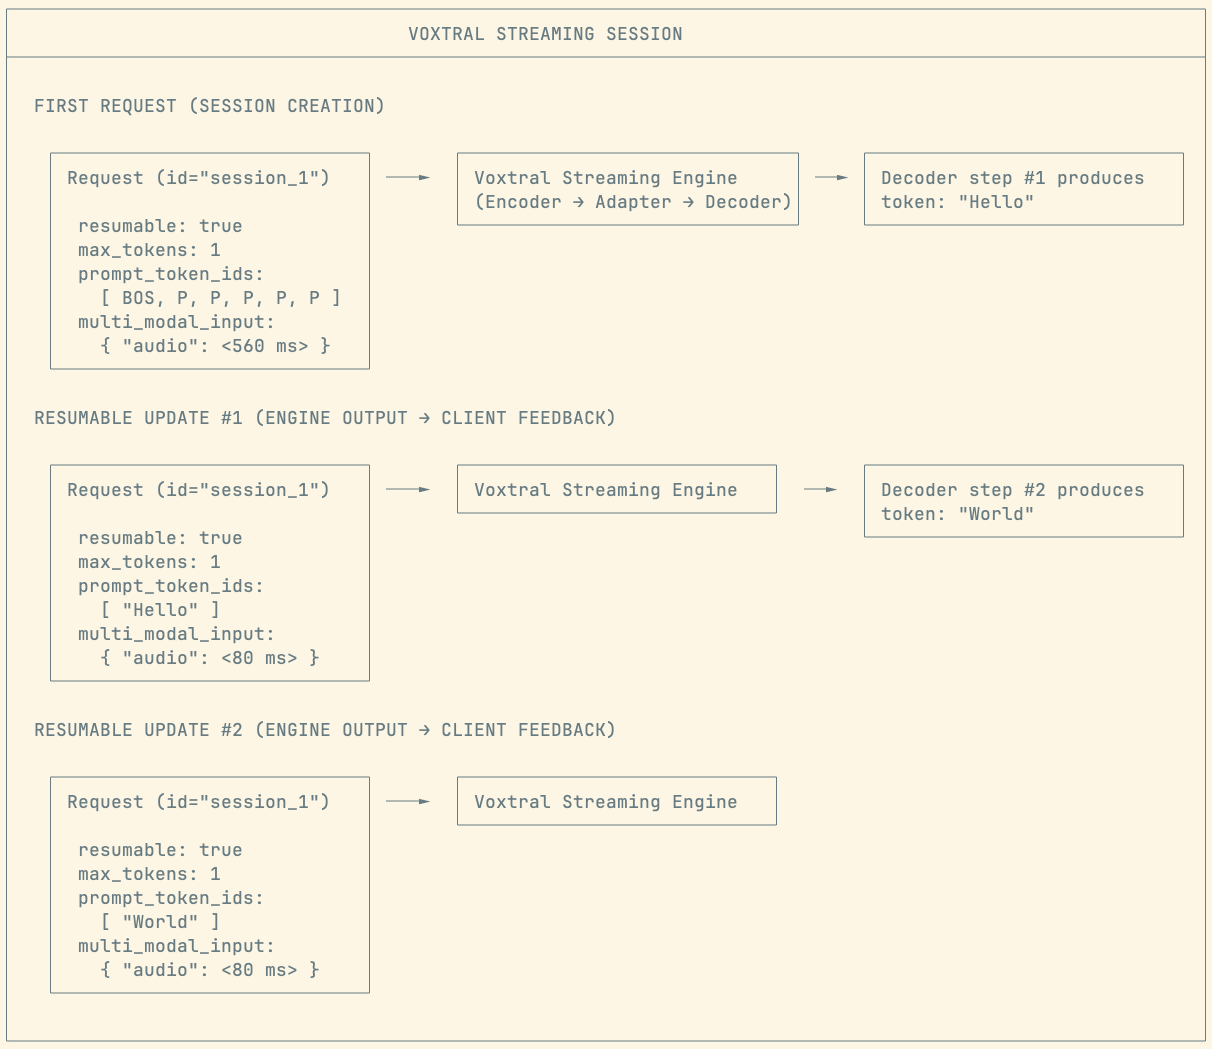
\includegraphics[width=\textwidth]{figures/vllm_session.png}
    \caption{\textbf{Voxtral streaming session via vLLM resumable requests.} A session is created with an anchor request that includes the initial buffered audio (e.g., the first $\tau$\,ms plus padding tokens to enforce the target delay) and runs a one-token decoder step. Each subsequent update is sent as a resumable request that appends the next 80\,ms audio chunk together with the previously emitted token ID, allowing the engine to reuse cached KV states and emit the next token incrementally. This request--decode--update loop enables low-latency, continuous transcription with full-duplex streaming-input/streaming-output.}
    \label{fig:vllm-session}
\end{figure}
